\documentclass[11pt,a4paper]{article}
\usepackage{graphicx}
\usepackage[T1]{fontenc}
\usepackage[utf8]{inputenc}
\usepackage{hyperref}
\usepackage{enumitem}
\usepackage{amsmath}

\title{Information Theory SV2}
\author{}
\date{}

% Style so question body appears below label
\setlist[enumerate,1]{label=\textbf{Question \arabic*:}, leftmargin=0pt,
  itemindent=! , labelsep=1em, align=left, labelwidth=*, listparindent=0pt}
\setlist[enumerate,2]{label=(\alph*), leftmargin=2em}
\setlist[enumerate,3]{label=(\roman*), leftmargin=3em}

\begin{document}
\maketitle

\emph{
\textbf{Question sources:} Matthew Ireland's SV worksheet, 23/24 Examples Sheet}

\begin{enumerate}

% Q1
\item  Explain why a terminating character is included in Arithmetic coding.  
    If it were not included, what information would you need to decode a message?  
    If it were included, what effect does the probability assigned to it have on the code?

    \item Consider a (7, 4) Hamming code which maps $k=4$ information bits to a length $n=7$ codeword.  
    Assume 0 and 1 are equiprobable in the input data.  

    Use the convention used by the rest of the world, not the one presented in lectures.  
    The transmitted codeword is \verb|[b1, b2, b3, b4, b5, b6, b7]| where:
    \[
    b_3, b_5, b_6, b_7 \text{ are the source bits,}
    \]
    \[
    b_4 = b_5 \oplus b_6 \oplus b_7, \quad
    b_2 = b_3 \oplus b_6 \oplus b_7, \quad
    b_1 = b_3 \oplus b_5 \oplus b_7.
    \]

    \begin{enumerate}
        \item Suppose that a codeword is transmitted over a binary symmetric channel (BSC), and the received codeword is  
        \verb|r = [1, 1, 0, 1, 0, 1, 1]|. Decode the received sequence to a codeword.

        \item Calculate the probability of block error $p_B$ of the (7, 4) Hamming code as a function of the bit error $p$ and show that to leading order it goes as $21p^2$.

        \item If the (7, 4) Hamming code can correct any one-bit error, might there be a (14, 8) code that can correct any two errors?
    \end{enumerate}

    \item Consider using the repetition code $R_5$ to encode binary input symbols for transmission through a binary symmetric channel with $f = 0.3$.  
    Assuming $p_0 < 0.5$, find the maximum value of $p_0$ for which the optimal decoder’s rule is not simply “pick the majority vote”.

    \item A binary symmetric channel receives as input a bit whose values $\{0,1\}$ have probabilities $\{p, 1-p\}$, but in either case, a transmission error can occur with probability $\varepsilon$, which flips the bit.  
    The surface plot describes the mutual information of this channel as a function $M(\varepsilon, p)$ of these probabilities:
    \begin{enumerate}
        \item At the point marked A, the error probability is $\varepsilon = 0$.  
        Why then is the channel mutual information minimal in this case: $M(\varepsilon, p) = 0$?

        \item At the point marked B, an error always occurs ($\varepsilon = 1$).  
        Why then is the channel mutual information maximal in this case: $M(\varepsilon, p) = 1$?

        \item At the point marked C, the input bit values are equiprobable ($p = 0.5$), so the symbol source has maximal entropy.  
        Why then is the channel mutual information in this case $M(\varepsilon, p) = 0$?
    \end{enumerate}

    \begin{figure}
        \centering
        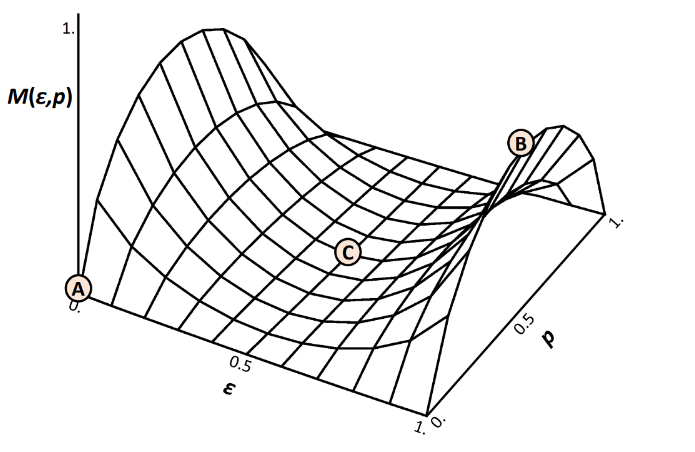
\includegraphics[width=0.7\linewidth]{tex/Screenshot 2024-11-18 194222.png}
        \label{fig:placeholder}
    \end{figure}

    \item (Mackay ex 6.4, p.119) Prove that any uniquely decodable code from $\{0,1\}^+$ to $\{0,1\}^+$ necessarily makes some strings longer if it makes some strings shorter.

    \item (Mackay ex 6.5, p.120) Encode the string \verb|000000000000100000000000| using the basic Lempel–Ziv algorithm.
\end{enumerate}


\end{document}
